\documentclass[a4paper, final]{article}

% ============================================================
% settings.tex
% ============================================================
\usepackage[russian]{babel}
\usepackage{fontspec}
\setmainfont{Times New Roman}
\newfontfamily\cyrillicfonttt{Courier New}
\usepackage[14pt]{extsizes}
\usepackage[left=20mm, top=20mm, right=20mm, bottom=20mm, footskip=10mm]{geometry}
\usepackage{ragged2e}
\usepackage{indentfirst}
\usepackage{graphicx}
\usepackage{tikz}
\usepackage{caption}
\usepackage{xcolor}
\usepackage{subcaption}
\usepackage{listings}
\usetikzlibrary{arrows.meta}
\usepackage{nccmath}
\usepackage{algorithm}
\usepackage{algorithmic}
\usepackage{booktabs}
\usepackage{hyperref}
\usepackage{pdflscape}
\usepackage{float}

\definecolor{link_color}{HTML}{0000EE}

\hypersetup{
    colorlinks=true,
    linkcolor=link_color,
    urlcolor=link_color,
    citecolor=link_color
}

\lstset{
    language=C++,
    basicstyle=\cyrillicfonttt\small,
    numbers=left,
    numberstyle=\tiny\color{gray},
    keywordstyle=\color{blue}\bfseries,
    commentstyle=\color{gray}\itshape,
    stringstyle=\color{red},
    frame=single,
    captionpos=b,
    breaklines=true,
    breakatwhitespace=false,
    showstringspaces=false,
    keepspaces=true,
    columns=flexible,
    fontadjust=true,
    basewidth={0.5em,0.45em},
    tabsize=4,
}

\begin{document}

% ============================================================
% title.tex
% ============================================================
{
\thispagestyle{empty}
\begin{center}
    \hfill \break
    \hfill \break
    МИНИСТЕРСТВО НАУКИ И ВЫСШЕГО ОБРАЗОВАНИЯ РОССИЙСКОЙ ФЕДЕРАЦИИ\\[5 pt]
    Федеральное государственное автономное образовательное учреждение высшего
    образования «Санкт-Петербургский политехнический университет Петра
    Великого»\\[10 pt]
    Институт компьютерных наук и кибербезопасности\\[5 pt]
    Направление: 02.03.01 Математика и компьютерные науки\\[30pt]

    {\large Отчет по дисциплине: «Теория графов»}\\[30 pt]
    \LARGE\bf «Разработка экспертных систем».
\end{center}

\vspace{110 pt}

\begin{tabular*}{460pt}{@{\extracolsep{\fill}} l r}
     Студент,\tabularnewline группы 5130201/40003 \hspace{50pt}
        & \line(1,0){100} \quad Адиатуллин Т. Р.\\
     & \\
     Руководитель,\tabularnewline Преподаватель
        & \line(1,0){121,5} \quad Востров А. В.\\
     & \\
     & \\
     & \\
     & \guillemotleft \line(1,0){30} \guillemotright
       \line(1,0){100} \, 2026 \,г.
\end{tabular*} \\

\vfill

\begin{center}
    Санкт-Петербург, 2026
\end{center}
\newpage
}

\tableofcontents
\newpage

\section*{Введение}
\addcontentsline{toc}{section}{Введение}

\justifying

Экспертные системы – это программы, имитирующие рассуждения специалиста в некоторой предметной области и позволяющие принимать решения там, где обычно требуется участие человека-эксперта. В отличие от традиционных алгоритмических программ, они основаны на эвристическом поиске решения и способны работать с неформализованными задачами. В рамках данной курсовой работы разработана экспертная система на базе языка CLIPS, которая помогает тренеру баскетбольной команды выбирать оптимальную тактику нападения в зависимости от игровой ситуации(фазы атаки, типа защиты соперника, структуры взаимодействий игроков и момента завершения эпизода.).

Целью работы является построение модели экспертной системы в виде би-
нарного дерева решений и её реализация средствами CLIPS. Дерево содержит
31 узел, 4 яруса и 15 терминальных узла (рекомендуемые модели автомоби-
лей).

\newpage

\section*{Постановка задач}
\addcontentsline{toc}{section}{Постановка задач}

\justifying

В рамках курсовой работы требуется разработать экспертную систему на языке CLIPS, реализующую продукционную модель представления знаний в виде бинарного дерева решений. Предметная область, тема и структура дерева согласованы с преподавателем. Минимальные требования к дереву: не менее 4 ярусов и не менее 30 узлов.
% В соответствии с заданием решались следующие задачи:
% \begin{enumerate}
%     \item Выбрать предметную область и формализовать критерии выбора тактики нападения.
%     \item Построить полное бинарное дерево решений не менее чем из 4 ярусов.
%     \item Реализовать дерево в CLIPS на основе продукционной модели знаний.
%     \item Реализовать диалог с пользователем с пошаговыми вопросами и ответами только в формате 1/2.
%     \item Обеспечить выдачу финальной рекомендации тактики на русском и английском языках.
% \end{enumerate}

\newpage

\section{Предметная область}

\justifying

Экспертная система предназначена для выбора оптимальной тактики нападения в баскетбольном матче на основе текущей игровой ситуации. Система анализирует фазу атаки, тип защиты соперника и действия игроков, задавая последовательность бинарных вопросов, и выдаёт рекомендацию по конкретному тактическому модальному (шаблону) завершения атаки.

Актуальность темы обусловлена высокой динамичностью современного баскетбола и необходимостью быстрой тактической адаптации. Согласно исследованию \cite{selmanović}, анализ структуры нападения позволяет определить модели высших достижений в профессиональном спорте. В ходе анализа 5718 игровых эпизодов в Евролиге и НБА было установлено, что, несмотря на различия в правилах, темп и динамика игры в обоих системах становятся всё более схожими. Обилие тактических вариантов (от быстрых прорывов до сложных позиционных взаимодействий) требует от тренера и игроков четкого понимания структуры нападения, что делает автоматизацию выбора тактики практически значимой задачей.

Выбор конкретной тактики определяется совокупностью факторов: стадией перехода (транзиции), численным преимуществом, типом защиты (личная или зонная) и спецификой взаимодействий (заслоны, рывки, игра спиной к кольцу). Эти критерии формируют узлы бинарного дерева решений, разделяя все атаки на первичные контратаки, вторичный прорыв и позиционное нападение.

\subsection{Обоснование таксономии тактик}

Все 16 тактических моделей, представленных в листьях дерева решений, являются фундаментальными единицами анализа структуры баскетбольного нападения. Классификация базируется на операциональных определениях исследования «Basic characteristics of offensive modalities in the Euroleague and the NBA». В системе тактики разделены на четыре основных блока в зависимости от фазы игры и типа защиты соперника.

\subsection{Первичное переходное нападение (Primary Transition)}

В этот блок входят тактики, реализуемые в первые секунды владения, часто при численном превосходстве или до того, как защита успела выстроиться.

\textbf{Primary transition} — классический быстрый прорыв, завершающийся организованным групповым взаимодействием в ранней фазе.

\textbf{1:1 facing the basket} — ситуация «один на один» лицом к кольцу, возникающая в переходе, когда атакующий использует скорость для обыгрыша защитника.

\textbf{Other offenses} — прочие варианты быстрых завершений, включая броски после вбрасывания или быстрые атаки после подбора, не попадающие в стандартные категории.

\textbf{1:1 back to basket} — завершение в раннем нападении через игрока, занимающего позицию спиной к корзине (пост), для использования преимущества в росте до прихода подстраховки.

\subsection{Вторичный прорыв и ранняя атака (Secondary Transition)}

Когда защита успела вернуться, но еще не организовала позиционную опеку, применяются тактики «второй волны».

\textbf{Pick and roll } — взаимодействие игрока с мячом и игрока, ставящего заслон, с последующим движением «большого» к кольцу. По данным~\cite{selmanović}, это самая частотная тактика в Евролиге.

\textbf{Pick \& Pop} — вариант заслона, при котором заслоняющий игрок уходит на периметр для дальнего броска.

\textbf{Spot-up} — бросок без ведения сразу после получения передачи. Критически важный элемент для реализации преимуществ, созданных партнерами.

\textbf{Early offense} — организованное нападение, начатое до того, как защита окончательно расставилась по местам и выбрала объекты опеки.

\subsection{Позиционное нападение против личной защиты}

В ситуациях установленной защиты (Man-to-Man) выбор тактики зависит от способа создания преимущества — индивидуально или через заслоны без мяча.

\textbf{Secondary transition} — переход в структурированную атаку, если первичные действия были остановлены, но мяч остается в активном движении.

\textbf{Set offense on man to man} — выполнение конкретной комбинации (сета) против личной защиты с четко распределенными ролями.

\textbf{Cut to/from basket} — тактика, основанная на рывках игроков без мяча в свободные зоны под кольцо или от него для получения паса.

\textbf{Handoff} — передача мяча из рук в руки, выполняющая роль «живого» заслона, позволяющая снайперу мгновенно освободиться для атаки.

\subsection{Комбинированное и зонное нападение}

Данный сегмент описывает тактики против специфических защитных построений или через ключевых игроков в «посту».

\textbf{Off-ball screen} — использование заслонов для игроков без мяча, обычно через «высокий пост», чтобы вывести снайпера на свободный бросок.

\textbf{Set offense} — стандартный позиционный розыгрыш через «низкий пост» (центрового), направленный на создание давления внутри трехсекундной зоны.

\textbf{Set offense on the zone - center} — атака против зонной защиты, организованная через центр (хай-пост или штрафную линию), чтобы «разбить» зону изнутри.

\textbf{Set offense on the zone - perimeter} — тактика против зоны, основанная на быстром движении мяча по периметру для поиска бреши в расстановке соперника.

\newpage


\section{Математическое описание}

\subsection{Экспертные системы}

Экспертные системы предназначены для решения неформализованных задач -- задач, характеризующихся ошибочностью, неточностью и неполнотой исходных данных, противоречивостью знаний о проблемной области, большой размерностью пространства решений и динамической изменчивостью данных непосредственно в процессе решения. В отличие от традиционных программ, ориентированных на исполнение известного алгоритма, экспертные системы основаны на эвристическом поиске решения, что позволяет им справляться с задачами, требующими знаний эксперта.

Экспертная система работает в двух режимах. В \textit{режиме приобретения знаний} эксперт при посредничестве инженера по знаниям наполняет систему данными, которые позволяют ей в дальнейшем решать задачи без его участия. В \textit{режиме консультации} конечный пользователь взаимодействует с системой напрямую, получая результат, не имея достаточных знаний в данной проблемной области.

Структура экспертной системы включает подсистему вывода, базу знаний, данные и модель представления данных, а также интеллектуальный редактор, через который эксперт совместно с инженером по знаниям наполняет систему.

\begin{figure}[h!]
  \centering
  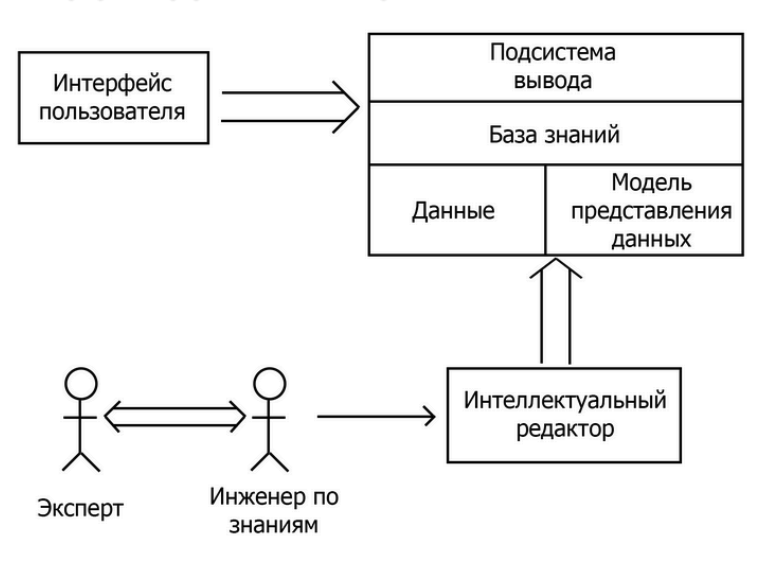
\includegraphics[width=0.7\textwidth]{Photo/struct.png}
  \caption{Структура экспертной системы}
  \label{fig:es_structure}
\end{figure}

\textbf{Знания} – это правила, законы и закономерности, полученные в результате профессиональной деятельности в пределах предметной области. \textbf{База знаний} – база данных, содержащая правила вывода и информацию о человеческом опыте и знаниях; иными словами, набор закономерностей, устанавливающих связи между вводимой и выводимой информацией. \textbf{Данные} – совокупность фактов и идей в формализованном виде. \textbf{Модель представления данных} – способ задания знаний для хранения, удобного доступа и взаимодействия с ними. 

Механизм логического вывода занимает наиболее важное место в структуре экспертной системы. Концептуально он представляется в виде <A, B, C, D>, где A – функция выбора закономерностей и фактов из базы знаний и базы данных соответственно; B – функция проверки правил, результатом которой определяется множество фактов, к которым применимы правила; C – функция, определяющая порядок применения правил при конфликте; D – функция, применяющая действие. Машина логического вывода выбирает правила, которым соответствуют факты, распределяет их по приоритетам и выполняет правило с наивысшим приоритетом.

\subsection{Продукционная модель}

Продукционная модель представления знаний близка к логическим моделям, что позволяет организовать эффективные процедуры логического вывода. Традиционная продукционная модель включает три базовых компонента: набор правил-продукций, образующих базу знаний; рабочую память, в которой хранятся исходные факты и факты, выведенные при помощи механизма вывода; сам механизм логического вывода, порождающий новые факты из имеющихся согласно правилам.

В основе продукционной модели лежит конструктивная единица -- продукция (правило):
\begin{lstlisting}[language={}, caption={}, nolol, frame=none, xleftmargin=0.3\textwidth]
IF условие THEN действие1 ELSE действие2
\end{lstlisting}

Продукция состоит из двух частей: условие называется антецедентом, действие -- консеквентом. Условия сочетаются с помощью логических функций AND и OR; антецеденты и консеквенты формируются из атрибутов и значений. Правило срабатывает, если при сопоставлении фактов рабочей памяти с антецедентом имеет место совпадение; результат заносится обратно в рабочую память.

\subsection{Бинарное дерево решений}

Бинарное дерево решений -- иерархическая структура, состоящая из узлов и ветвей. Корневой узел содержит начальный вопрос. \textit{Внутренние узлы} представляют собой вопросы, используемые для разбиения. \textit{Ветви} соединяют узлы и представляют возможные ответы. \textit{Листовые (терминальные) узлы} содержат окончательное решение.

Каждый путь от корня к листу соответствует одному продукционному правилу: промежуточные узлы формируют антецедент, лист -- консеквент. Для полного бинарного дерева глубиной $d$ выполняются следующие соотношения:
\begin{itemize}
    \item количество листьев: $2^d$;
    \item количество внутренних узлов: $2^d - 1$;
    \item общее количество узлов: $2^{d+1} - 1$;
    \item количество рёбер: $2^{d+1} - 2$.
\end{itemize}

В настоящей работе построено полное бинарное дерево глубиной $d = 4$ (ярусы $0$--$4$):
\[
    2^{4+1} - 1 = 31 \text{ узел}, \quad 2^4 = 16 \text{ листьев}, \quad 2^4 - 1 = 15 \text{ внутренних узлов}.
\]

Поиск решения начинается с корневого узла. В каждом узле анализируется вопрос, в зависимости от ответа выбирается одна из двух ветвей и происходит переход к следующему узлу. Шаги повторяются до достижения листового узла.

\begin{landscape}
  \thispagestyle{empty}
  \captionsetup{font=small,skip=4pt}

  \begin{figure}[!p]
    \centering
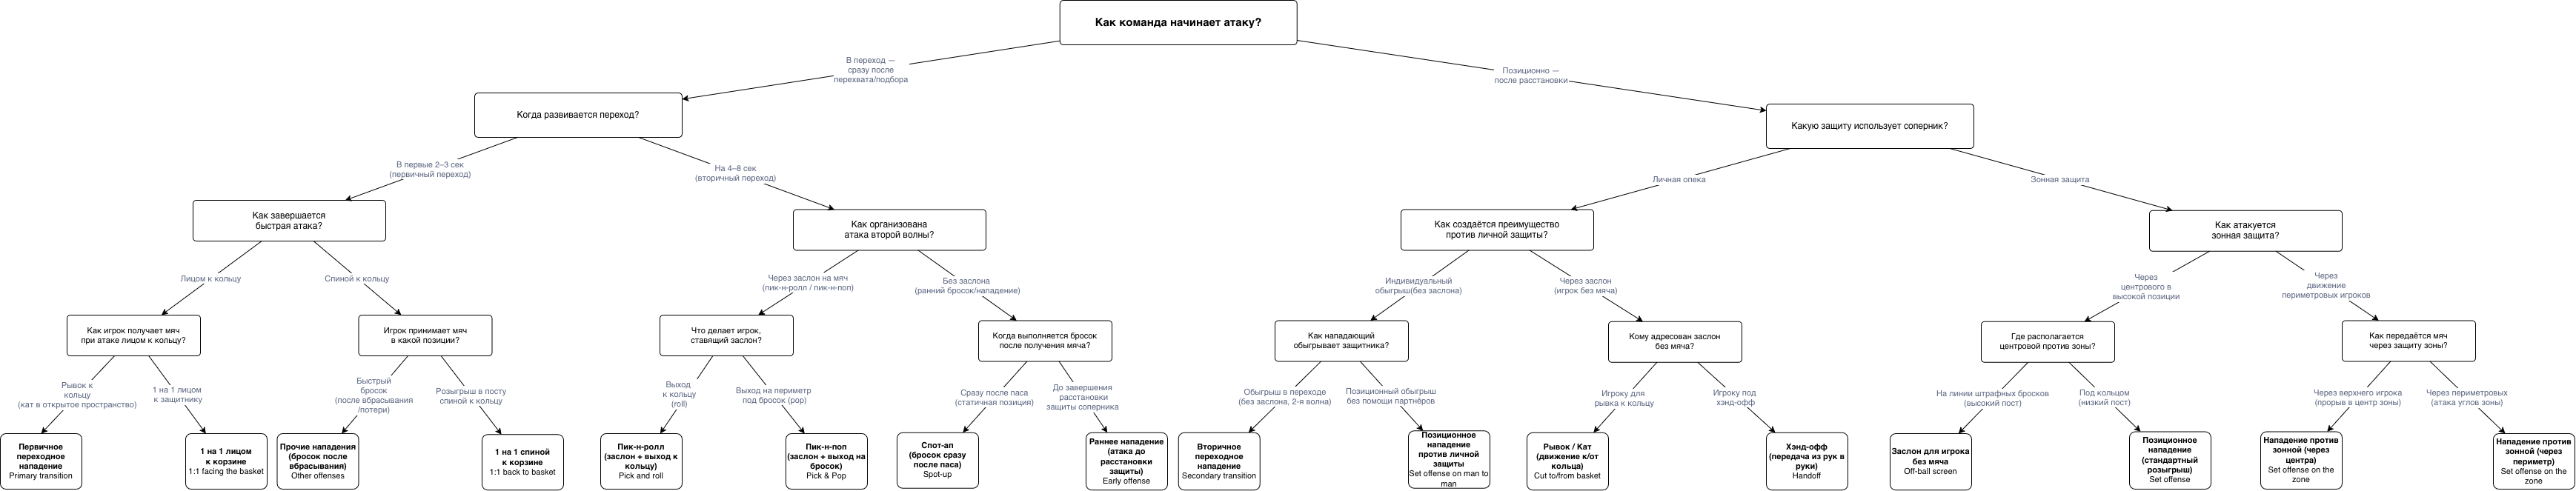
\includegraphics[width=\linewidth,height=\dimexpr\textheight-4\baselineskip\relax,keepaspectratio]{Photo/tgraph_diag.png}
    \caption{Правое поддерево всего бинарного дерева}
    \label{fig:right}
  \end{figure}
\end{landscape}

\restoregeometry
\clearpage

\subsection{Среда разработки CLIPS}

Реализация выполнена в среде CLIPS (C Language Integrated Production System) -- инструменте построения экспертных систем на основе продукционной модели представления знаний.

В проекте используются ключевые конструкции CLIPS:
\begin{itemize}
    \item \texttt{deftemplate} -- объявление шаблона факта;
    \item \texttt{deffunction} -- объявление пользовательской функции;
    \item \texttt{defrule} -- объявление правила;
    \item \texttt{assert} -- добавление факта в рабочую память;
    \item \texttt{not} -- проверка отсутствия факта;
    \item \texttt{halt} -- остановка вывода после получения конечной рекомендации.
\end{itemize}

В данной работе используется версия CLIPS~6.4.2 (см. рисунок ~\ref{fig:version}).

\begin{figure}[h!]
  \centering
  
\includegraphics[width=0.7\textwidth]{Photo/clips.jpg}
  \caption{Версия CLIPS}
  \label{fig:version}
\end{figure}

\newpage

\section{Особенности реализации}

\justifying

Экспертная система реализована в одном файле \texttt{expert\_basketball.clp}. Логика системы полностью соответствует дереву решений из 15 вопросов и 16 конечных тактик.

\subsection{Определение шаблонов и функций}

Для хранения ответов используется шаблон факта \texttt{attr} с двумя слотами: \texttt{name} и \texttt{val}. После каждого ответа пользователя в рабочую память добавляется факт вида \texttt{(attr (name ... ) (val ... ))}.

Функция \texttt{ask-choice} реализует диалог с пользователем: выводит текст вопроса и два варианта ответа, принимает только числа 1 или 2, а затем возвращает соответствующее символьное значение ветви.

\begin{lstlisting}[caption={Шаблон и функция чтения ответа}]
(deftemplate attr
  (slot name)
  (slot val))

(deffunction ask-choice (?question ?v1 ?d1 ?v2 ?d2)
  (printout t crlf ?question crlf)
  (printout t "  1 - " ?d1 crlf)
  (printout t "  2 - " ?d2 crlf)
  (printout t "Ваш выбор (1/2): ")
  (bind ?ans (read))
  (while (and (neq ?ans 1) (neq ?ans 2)) do
    (printout t "Введите только 1 или 2: ")
    (bind ?ans (read)))
  (if (eq ?ans 1) then ?v1 else ?v2))
\end{lstlisting}

\subsection{Правила}

Каждый внутренний узел дерева реализован правилом-вопросом \texttt{q*}. Антецедент содержит путь от корня и условие отсутствия текущего факта. Консеквент вызывает \texttt{ask-choice} и добавляет следующий факт в рабочую память.

\begin{lstlisting}[caption={Пример правила-вопроса (узел 8)}]
(defrule q8-poziciya-priema-myaca
  (attr (name nacalo-ataki) (val perehod))
  (attr (name tempo-perehoda) (val pervichniy))
  (attr (name zavershenie-bystroy-ataki) (val spinoy))
  (not (attr (name poziciya-priema-myaca)))
  =>
  (bind ?ans (ask-choice
    "Игрок принимает мяч в какой позиции?"
    bystry-brosok "Быстрый бросок (после вбрасывания/потери)"
    post "Розыгрыш в посту спиной к кольцу"))
  (assert (attr (name poziciya-priema-myaca) (val ?ans))))
\end{lstlisting}

Каждый лист реализован отдельным правилом \texttt{leaf-*}. В правиле листа проверяется полный путь (4 ответа), после чего система выводит название тактики на русском и английском языках и завершает работу через \texttt{halt}.

\begin{lstlisting}[caption={Пример факта (лист 1 - Первичное переходное нападение)}]
(defrule leaf-01
  (attr (name nacalo-ataki) (val perehod))
  (attr (name tempo-perehoda) (val pervichniy))
  (attr (name zavershenie-bystroy-ataki) (val licom))
  (attr (name sposob-polucheniya-myaca-licom) (val kat))
  =>
  (printout t crlf "Первичное переходное нападение (Primary transtion)" crlf)
  (halt))
\end{lstlisting}

\subsection{Логика работы}

После загрузки файла и запуска \texttt{(reset)} + \texttt{(run)} система:
\begin{enumerate}
    \item выводит заголовок экспертной системы;
    \item последовательно задаёт 4 вопроса по одному;
    \item на каждом шаге принимает только ответ 1 или 2;
    \item после достижения листа выдаёт итоговую тактику.
\end{enumerate}

\newpage

\section{Результаты работы программы}

\justifying

Программа успешно отрабатывает все пути дерева и всегда выдаёт одну тактику, соответствующую введённой комбинации ответов.

Пример получения Spot-up (лист 7) показан на рисунке~\ref{fig:tac1}.
\begin{figure}[H]
  \centering
  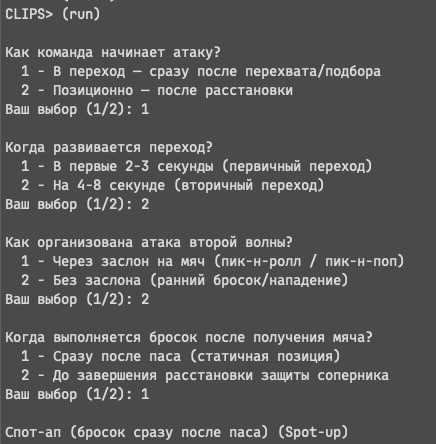
\includegraphics[width=0.7\textwidth]{Photo/tac1.jpg}
  \caption{Пример сценария получения рекомендации тактики №1}
  \label{fig:tac1}
\end{figure}

 Пример получения Cut to/from basket (лист 11) -- на рисунке~\ref{fig:tac2}.

\begin{figure}[H]
  \centering
  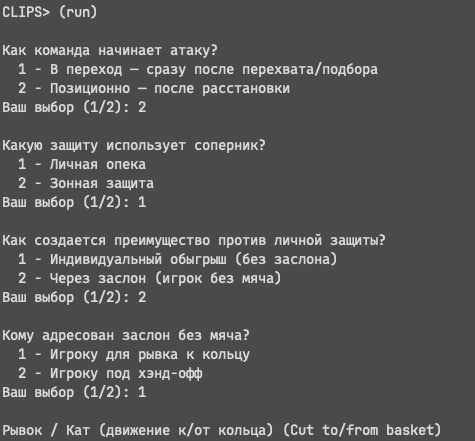
\includegraphics[width=0.7\textwidth]{Photo/tac2.jpg}
  \caption{Пример сценария получения рекомендации тактики №2}
  \label{fig:tac2}
\end{figure}

На рисунке~\ref{fig:uncurr} показано, что при некорректном вводе (например, 3) система запрашивает повторный ввод до получения допустимого ответа.

\begin{figure}[H]
  \centering
  
\includegraphics[width=0.7\textwidth]{Photo/uncurr.jpg}
  \caption{Пример некорректного ввода и его обработка}
  \label{fig:uncurr}
\end{figure}


\newpage

\section*{Заключение}
\addcontentsline{toc}{section}{Заключение}

\justifying

В ходе работы была построена модель экспертной системы выбора тактик баскетбольно команды в виде бинарного дерева решений и её реализация средствами CLIPS. Дерево содержит
31 узел, 4 яруса и 15 терминальных узла (рекомендуемые модели автомоби-
лей).

\subsection*{Реализованный функционал}
Построено полное бинарное дерево решений на 31 узел (15 вопросов и 16 листьев). Реализована база знаний в CLIPS в виде правил-вопросов и правил-результатов. Реализован интерактивный опрос пользователя с валидацией ответов (только 1/2). Для каждого пути дерева выдаётся однозначная тактика на русском и английском языках.

\subsection*{Достоинства реализации}
Простая и прозрачная логика вывода, каждый путь от корня к листу легко интерпретируется. После фиксированного числа шагов система всегда приходит к одному результату. Добавление или корректировка тактик выполняется через редактирование правил.

\subsection*{Недостатки реализации}
Жёсткая бинарность вопросов ограничивает гибкость описания игровых ситуаций. Нет учёта вероятностных/нечётких факторов (текущей формы игроков, контекста матча, статистики владений). Модель не объясняет альтернативы, а выдаёт только один конечный вариант тактики.

\subsection*{Масштабирование}
Разработка графического интерфейса и экспорт рекомендаций в формат тренерских сценариев.

\newpage

% ============================================================
% Список литературы
% ============================================================
\begin{thebibliography}{99}

\bibitem{telematika}
Секция «Телематика» [Электронный ресурс]. ---
URL: \url{https://tema.spbstu.ru/tgraph/} (дата обращения: 16.05.2026).

\bibitem{selmanović}
\textit{Selmanović, Škegro, Milanović (2015) — «Basic characteristics of basketball offense modalities in the Euroleague and the NBA»}
URL: \url{https://www.breakthroughbasketball.com/offense/5-out-offense-away-tipton}
(дата обращения: 10.05.2026).

\bibitem{clips}
\textit{CLIPS Rule Based Programming Language // SourceForge.}
URL: \url{https://sourceforge.net/projects/clipsrules}
(дата обращения: 10.05.2026)

\bibitem{gavril}
\textit{Гаврилова Т. А., Частиков А. П. Разработка экспертных систем. Среда
CLIPS. — СПб.: БХВ-Петербург, 2003. — 608 с.}
(дата обращения: 10.05.2026)..


\end{thebibliography}

\newpage

\section*{Приложение. Листинг программы}
\addcontentsline{toc}{section}{Приложение. Листинг программы}

\lstinputlisting[
  language={},
  caption={Листинг экспертной системы выбора тактики (\texttt{expert\_basketball.clp})}
]{../expert_basketball.clp}

\end{document}